\section{Rigid Bodies}

\begin{definition}[Rigid body]
    A \textbf{rigid body} is an extended object, consisting of $N$ particles that are constrained such that the distance between any pair of particles, $|\mathbf{r}_i - \mathbf{r}_j|$, is fixed. 
\end{definition}

The possible motions of a rigid body are the continuous isometries of Euclidean space, i.e. translations and rotations. Reflections change the ordering of intrisic structure of the rigid body so they are not included.

\subsection{Angular velocity}

Recall that if a particle is rotating about an axis through $O$ with angular velocity $ \boldsymbol{\omega} $ then the velocity $ \dot{\bfr} = \boldsymbol{\omega}\times \bfr $ with $ |\dot{\bfr}|=\omega r_\perp  $, where $ r_\perp  $ is the perpendicular distance to the axis of rotation.

If the particle has mass $m$, then the kinetic energy $T$ is 
\[
    T = \frac{1}{2}m|\dot{\mathbf{r}}|^2 = \frac{1}{2}m (\boldsymbol{\omega}\times \bfr)\cdot (\boldsymbol{\omega}\times \bfr) = \frac{1}{2}{\color{blue}mr_\perp^2} \omega^2 = \frac{1}{2}{\color{blue}I} \omega^2 .
\]
\begin{note}
    If $ \boldsymbol{\omega}=\omega \bfn $ then $ r_\perp = |\mathbf{n}\times \mathbf{r}| $.
\end{note}

\begin{definition}[Moment of inertia]
    The \textbf{moment of inertia} of a particle is
    \[
      I = m r_\perp^2 = m|\mathbf{n}\times \mathbf{r}|^2,
    \]
\end{definition}

\subsection{Moment of inertia}

Consider a rigid body made up of $N$ particles. Consider the body to be rotating about an axis through the origin with angular velocity $ \boldsymbol{\omega} $. Then for each particle 
\[
    \dot{\mathbf{r}}_i = \boldsymbol\omega\times \mathbf{r}_i.
\]
This ensures $ |\mathbf{r}_i-\mathbf{r}_j| $ does not vary with time:
\[
  \frac{\rmd }{\rmd t}|\mathbf{r}_i - \mathbf{r}_j|^2 = 2(\dot{\mathbf{r}}_i - \dot{\mathbf{r}}_j)\cdot (\mathbf{r}_i - \mathbf{r}_j) = 2\big(\boldsymbol\omega\times (\mathbf{r}_i - \mathbf{r}_j)\big) \cdot (\mathbf{r}_i - \mathbf{r}_j) = 0,
\]

Similarly, the kinetic energy is
\[
  T = \frac{1}{2}\sum_{i = 1}^N m_i|\dot{\mathbf{r}_i}|^2 =\frac{1}{2}\sum_{i = 1}^N m_i |\boldsymbol\omega\times \mathbf{r}_i|^2 = \frac{1}{2}\omega^2 {\color{blue}\sum_{i = 1}^N m_i  |\bfn \times \bfr_i|^2} = \frac{1}{2}{\color{blue}I}\omega^2.
\]
\begin{definition}[Moment of inertia]
    The \textbf{moment of inertia} of a rigid body about the rotation axis $\mathbf{n}$ is
    \[
      I = \sum_{i = 1}^N m_i(r_i)_{\perp}^2 = \sum_{i = 1}^N m_i  |\bfn \times \bfr_i|^2.
    \]
\end{definition}
\begin{definition}[Angular momentum]
    The \textbf{angular momentum} is
    \[
      \mathbf{L} = \sum_{i=1}^N m_i \mathbf{r}_i \times \dot{\mathbf{r}}_i = \sum_{i=1}^N m_i \mathbf{r}_i \times \boldsymbol\omega \times \mathbf{r}_i.
    \]
\end{definition}

Consider $ \boldsymbol{\omega}=\omega \mathbf{n} $, then 
\[
    \mathbf{L} = \omega \sum_{i=1}^N m_i (\mathbf{r}_i \times (\mathbf{n} \times \mathbf{r}_i)).
\]
Consider the part of $ \bfL $ parallel to the rotation of axis: 
\begin{align*}
    \mathbf{L} \cdot \mathbf{n} &= \omega \sum_{i=1}^N m_i \mathbf{n}\cdot (\mathbf{r}_i \times (\mathbf{n} \times \mathbf{r}_i))\\
    &= \omega \sum_{i=1}^N m_i(\mathbf{n}\times \mathbf{r}_i)\cdot (\mathbf{n} \times \mathbf{r}_i)\\
    &= \omega \sum_{i=1}^{N}m_i(r_i)_{\perp}^2 = I\omega.
\end{align*}
So component of angular momentum in direction of rotation axis is $ I \omega $. In general $ \mathbf{L} $ is \textit{not} $\parallel$ to rotation axis. But we can write 
\[
  \mathbf{L} = \sum_{i=1}^N m_i\big((\mathbf{r}_i\cdot \mathbf{r}_i)\boldsymbol \omega - (\mathbf{r}_i \cdot \boldsymbol\omega)\mathbf{r}_i\big),
\]
which is linear of $\boldsymbol\omega$. So we can write
\[
  \mathbf{L} = I \cdot \boldsymbol \omega,
\]
where we abuse notation to use $I$ for the \textbf{inertia tensor}. In suffix notation $ L_i = I_{ij}\omega_j $. Note that $I$ is a \textit{symmetric} tensor with components
\[
  I_{jk} = \sum_{i=1}^N m_i(|\mathbf{r}_i|^2 \delta_{jk} - (\mathbf{r}_i)_j(\mathbf{r}_i)_k),
\]
In general, there are 3 directions such that $ I \boldsymbol{\omega} \parallel \boldsymbol{\omega} $, which corresponds to \textbf{principal axes} of the tensor. If the body is rotated about a principal axis, then $\mathbf{L}\parallel \boldsymbol\omega$. Note that it holds for \textit{any} body.

Recap the simple case: if we choose to rotate in a direction such that $ \mathbf{L}\parallel \boldsymbol\omega $, then 
\[
    \bfL = I(\bfn) \boldsymbol{\omega},
\]
where $ I(\bfn) $ is the moment of inertia about $\bfn$. We often consider bodies that are \textit{symmetric} about a particular axis, and rotating about that axis guarantees above property. 

\subsection{Calculation of the moment of inertia}
For a solid body, we replace mass-weighted sums over particles by mass-weighted integrals. In particular, consider a body occupying a volumn $V$ with the mass density $\rho(\mathbf{r})$. Then 
\begin{definition}
    The \textbf{mass} is
    \[
      M = \int_V \rho(\mathbf{r}) \,\rmd V.
    \]
    The \textbf{centre of mass} is
    \[
      \mathbf{R} = \frac{1}{M}\int_V \mathbf{r}\rho(\mathbf{r})\,\rmd V.
    \]
    The \textbf{moment of inertia} about axis $\bfn$ is
    \[
      I = \int_V \rho(\mathbf{r}) r_{\perp}^2 \,\rmd V = \int_V \rho(\mathbf{r})|\mathbf{n}\times \mathbf{r}|^2\,\rmd V.
    \]
\end{definition}
Use the obvious modifications of these formulae for bodies that corresponds to mass distributed over a surface or along a curve, as surface(area) integrals or line integrals.

\begin{example}
    Consider a uniform ring of mass $M$ and radius $a$, about an axis through the center, perpendicular to the plane of the ring.
    \begin{center}
      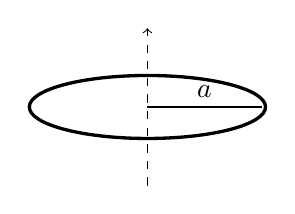
\begin{tikzpicture}
        \draw [dashed,->] (0, -1) -- (0, 1);
        \draw [very thick] circle [x radius = 1.5, y radius = 0.4];
        \draw (0, 0) -- (1.45, 0) node [pos = 0.5, above] {$a$};
      \end{tikzpicture}
    \end{center}
    In this case we reduce to a line integral and $ \rho = M/2\pi a $. $ r_{\perp }=a $, so 
    \[
      I = \int_{0}^{2\pi} \underbrace{\frac{M}{2\pi a}}_{\rho} \underbrace{a^2}_{r_{\perp}^2} \underbrace{a \dd \theta}_{\rmd s}= Ma^2.
    \]
\end{example}

\begin{example}
    Consider a uniform rod of mass $M$ and length $l$ with axis through one end, perpendicular to the rod.
    \begin{center}
      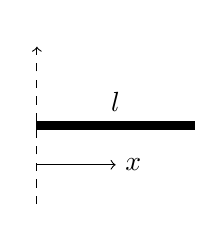
\begin{tikzpicture}
        \draw [dashed,->] (0, -1) -- (0, 1) node [above] {$\bfn$};
        \filldraw[black] (0, 0.05) rectangle (2, -0.05);
        \node at (1, 0.3) {$l$};
        \draw [->] (0,-0.5) -- (1,-0.5) node [right] {$x$};
      \end{tikzpicture}
    \end{center}
    $\rho = M/l$. So the moment of inertia is
    \[
      I = \int_0 ^l \frac{M}{l}x^2\dd x = \frac{1}{3}Ml^2.
    \]
\end{example}